\section{Results Across Four Reporting Levels}
\label{sec:results}

The previous section evaluates the analysis methods. This section presents the saved outputs at four levels: one company, selected companies in one sector, the full financial-sector group, and all recorded sectors. All company values come from the saved exports. The examples connect passage-level analysis with company scores and sector summaries.

The saved database contains 1,164 company records and 1,172 filing records. The score export has one row for each of 1,164 unique CINs, using the most recent available filing selected by the script. These counts define the company collection used in the reporting examples.

\subsection{One company: from filed facts to an interpretable outcome}
\label{sec:case}

Triveni Turbine Limited is a worked example with all four score components and a sector comparison. The linked database filing ends on 31 March 2026 and contains 1,862 raw facts. Table~\ref{tab:case_facts} shows three previous/current value pairs with matching concepts, units, and periods. Scope 1 emissions rise, Scope 2 emissions fall, and water withdrawal falls. These different directions show why one general claim of environmental improvement cannot be compared with every environmental figure.

\begin{table}[tbp]
\centering\small
\caption{Filed values for Triveni Turbine, copied from filing record 197 without correction. Concept, period, and unit links allow the pairs to be checked. The source links identify the original company values.}
\label{tab:case_facts}
\begin{tabularx}{\linewidth}{@{}Yrrl@{}}
\toprule\textbf{Filed measure} & \textbf{FY2024--25} & \textbf{FY2025--26} & \textbf{Filed unit}\\\midrule
Scope 1 emissions & 4,142.84 & 5,177.03 & tCO2e\\
Scope 2 emissions & 3,353.61 & 3,169.15 & tCO2e\\
Total water withdrawal & 88,662.28 & 85,611.54 & Kilolitres\\\bottomrule
\end{tabularx}
\end{table}

The workflow stores the figures beside narrative facts and reporting categories. An eligible passage receives a principle label from an explicit tag, concept map, or principle note. The classifier ranks the nine principles, and the language detector identifies evidence markers and vague wording. Numerical checks retrieve the value pairs in Table~\ref{tab:case_facts}. The worked example presents the saved facts and score components for this filing.

Every part of the saved score can be explained. The filing has 613 accepted concepts out of 1,057 in the database, giving Completeness of $100(613/1057)=57.99\%$. Scoring retains 52 concept--text pairs. Specificity of 63.46\% corresponds to 33 of 52 passages with a recognised evidence pattern. Clarity of 98.08\% corresponds to one flagged passage and 51 without a flag. SDG breadth of 70.59\% corresponds to 12 of the 17 goals under the fixed map. These counts reproduce the saved component percentages.

\begin{table}[tbp]
\centering\small
\caption{Transparency Score calculation for Triveni Turbine. Each percentage is multiplied by the weight. The final column shows the contribution before rounding the total.}
\label{tab:case_score}
\begin{tabularx}{\linewidth}{@{}Yrrr@{}}
\toprule\textbf{Component} & \textbf{Percentage} & \textbf{Weight} & \textbf{Contribution}\\\midrule
Completeness & 57.99 & 0.40 & 23.196\\
Specificity & 63.46 & 0.30 & 19.038\\
Clarity & 98.08 & 0.20 & 19.616\\
SDG breadth & 70.59 & 0.10 & 7.059\\\midrule
\textbf{Transparency Score} & & & \textbf{68.91}\\\bottomrule
\end{tabularx}
\end{table}

Equation~\eqref{eq:ts} gives $23.196+19.038+19.616+7.059=68.909$, rounded to 68.91. Figure~\ref{fig:company_contributions} plots each weighted contribution. The Machinery and Equipment group contains 36 companies with mean score 49.46. Triveni's percentile of 94.4 places the filing near the upper end of this recorded peer group.

\begin{figure}[tbp]
\centering
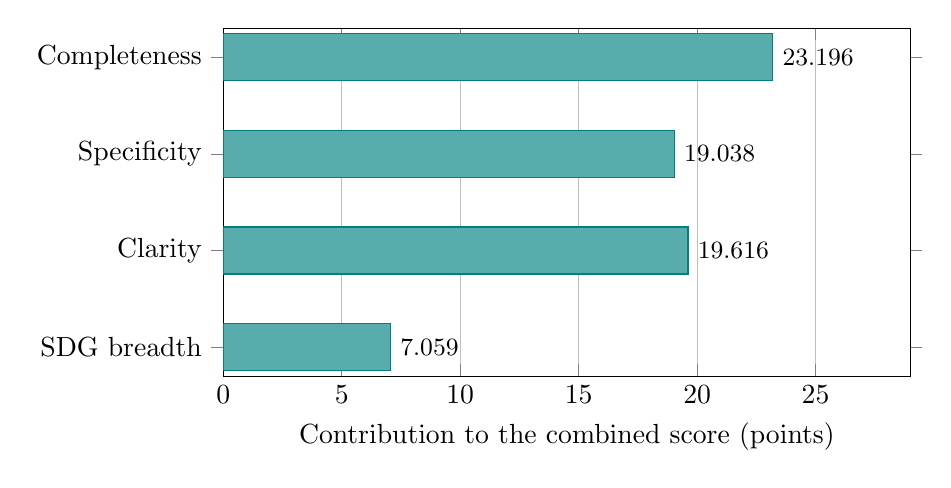
\begin{tikzpicture}
\begin{axis}[width=0.85\linewidth,height=6cm,xbar,bar width=17pt,
  xlabel={Contribution to the combined score (points)},xmin=0,xmax=29,
  symbolic y coords={SDG breadth,Clarity,Specificity,Completeness},ytick=data,xmajorgrids=true,
  nodes near coords,nodes near coords style={font=\small,/pgf/number format/fixed,/pgf/number format/precision=3}]
\addplot[fill=teal!65,draw=teal] coordinates {(7.059,SDG breadth)(19.616,Clarity)(19.038,Specificity)(23.196,Completeness)};
\end{axis}
\end{tikzpicture}
\caption{How the Triveni Turbine score is calculated. Each bar is the component percentage multiplied by the fixed weight. Completeness adds 23.196 points, Specificity 19.038, Clarity 19.616, and SDG breadth 7.059. The total is 68.909, rounded to 68.91. The bars show each component's contribution to the combined score.}
\label{fig:company_contributions}
\end{figure}

\FloatBarrier

\subsection{Selected financial companies: component differences and available years}
\label{sec:selected_finance}

The second level compares companies within one recorded sector. The saved \emph{Financial Services (excl. Insurance)} group has 94 companies. Table~\ref{tab:financial_selected} shows the four highest and three lowest scores. These examples show the range and are not a random sample. The next level summarises the full group.

\begin{table}[tbp]
\centering\small
\caption{Financial-company examples from the high and low ends of the score range. FY end 2026 and 2025 mean 31 March of those years. $C$, $Sp$, $Cl$, and $G$ are percentages; TS is the combined score. Years were reconstructed from the latest filing for each CIN.}
\label{tab:financial_selected}
\begin{tabularx}{\linewidth}{@{}Yrrrrrr@{}}
\toprule\textbf{Company} & \textbf{FY end} & \textbf{$C$} & \textbf{$Sp$} & \textbf{$Cl$} & \textbf{$G$} & \textbf{TS}\\\midrule
REC & 2026 & 56.01 & 57.69 & 98.08 & 82.35 & 67.56 \\
Mahindra \& Mahindra Financial Services & 2026 & 67.83 & 49.15 & 98.31 & 29.41 & 64.48 \\
YES BANK & 2026 & 60.45 & 46.67 & 92.00 & 70.59 & 63.64 \\
KOTAK MAHINDRA BANK & 2026 & 61.21 & 59.42 & 95.65 & 17.65 & 63.21 \\
Fedbank Financial Services & 2025 & 31.98 & 12.12 & 75.76 & 0.00 & 31.58 \\
Nalwa Sons Investments & 2025 & 31.13 & 10.26 & 74.36 & 0.00 & 30.40 \\
Vardhman Holdings & 2025 & 35.00 & 2.78 & 75.00 & 0.00 & 29.83 \\
\bottomrule
\end{tabularx}
\end{table}

REC Limited scores 67.56 and Vardhman Holdings scores 29.83. Specificity is 57.69\% for REC and 2.78\% for Vardhman; Completeness is 56.01\% and 35.00\%. The component view shows where the disclosures differ under the same formula. Review also uses the business model, recorded sector, applicable reporting items, and available filing year to interpret the comparison.

A year comparison uses repeated filings for the same company. For ESAF Small Finance Bank, Completeness rises from 34.34\% to 54.59\%, Specificity from 30.23\% to 41.30\%, and Clarity from 93.02\% to 93.48\%. SDG breadth stays at 11.76\%. The combined score rises from 42.59 to 54.10, or 11.51 points. Completeness contributes about 8.10 points, Specificity 3.32 points, and Clarity 0.09 points. The breakdown connects each component change to the reported score movement.

Table~\ref{tab:esaf} presents all eight companies with two available years. Six scores rise and two fall. The group mean rises from 45.17 to 50.40, a change of 5.23 points. The final column gives the component with the largest absolute weighted contribution to each change. Contributions from other components complete the total. Supplementary Table S3 retains both filing records, year labels, and every component for the eight-company group.

\begin{table}[tbp]
\centering\small
\caption{Two-year Transparency Scores for all eight available companies. Changes and weighted contributions are score points. $C$, $Sp$, $Cl$, and $G$ are defined in Eq.~\eqref{eq:ts}. The last column gives the component with the largest absolute contribution to the change.}
\label{tab:esaf}
\begin{tabularx}{\linewidth}{@{}Yrrrr@{}}
\toprule\textbf{Company} & \textbf{FY2024--25} & \textbf{FY2025--26} & \textbf{Change} & \textbf{Largest contribution}\\\midrule
Praj Industries & 38.55 & 50.30 & +11.75 & $C$: +9.91 \\
ESAF Small Finance Bank & 42.59 & 54.10 & +11.51 & $C$: +8.10 \\
Sudarshan Colorants & 49.74 & 58.78 & +9.04 & $Sp$: +7.00 \\
Gopal Snacks & 41.30 & 47.29 & +5.99 & $Sp$: +8.53 \\
G R Infraprojects & 35.94 & 38.87 & +2.93 & $Sp$: +3.07 \\
Sudarshan Chemical & 62.95 & 65.32 & +2.37 & $G$: +2.35 \\
VIP Industries & 45.91 & 45.56 & -0.35 & $Cl$: -2.36 \\
SML Mahindra & 44.38 & 42.98 & -1.40 & $Cl$: -1.17 \\
\midrule
Group mean & 45.17 & 50.40 & +5.23 & \na\\\bottomrule
\end{tabularx}
\end{table}

\subsection{The complete financial-sector group}
\label{sec:all_finance}

For all 94 financial-sector companies, the mean is 48.17, the median is 49.79, and the standard deviation is 9.88. Scores range from 29.83 to 67.56, a spread of 37.73 points. Mean Completeness is 49.77\%, Specificity 28.35\%, Clarity 90.67\%, and SDG breadth 16.27\%. Clarity is much higher than Specificity. This difference shows why avoiding vague phrases alone does not provide concrete evidence.

The latest recorded filing ends in March 2026 for 77 companies and March 2025 for 17. Year labels were reconstructed by CIN from the database using the script's latest-filing rule; the original score CSV omits a filing identifier. The group is a latest-available filing collection. The separate eight-company comparison uses paired reports to examine year-wise score changes.

\begin{table}[tbp]
\centering\small
\caption{All 94 financial companies grouped by score. Each company appears in one band. Component columns give mean percentages; TS gives the mean combined score. Supplementary Table S1 lists every company, reconstructed filing year, and sector percentile.}
\label{tab:all_financial}
\begin{tabularx}{\linewidth}{@{}Yrrrrrrr@{}}
\toprule\textbf{Score band} & \textbf{N} & \textbf{Mean TS} & \textbf{Range} & \textbf{$C$} & \textbf{$Sp$} & \textbf{$Cl$} & \textbf{$G$}\\\midrule
60.00--69.99 & 11 & 62.39 & 60.01--67.56 & 61.17 & 47.24 & 95.25 & 47.06 \\
50.00--59.99 & 35 & 54.77 & 50.23--59.84 & 60.69 & 32.94 & 94.07 & 17.98 \\
40.00--49.99 & 26 & 45.22 & 40.57--49.96 & 45.85 & 26.05 & 89.79 & 11.08 \\
Below 40.00 & 22 & 34.05 & 29.83--39.80 & 31.33 & 14.30 & 84.02 & 4.28 \\
\midrule
All financial companies & 94 & 48.17 & 29.83--67.56 & 49.77 & 28.35 & 90.67 & 16.27\\\bottomrule
\end{tabularx}
\end{table}

Table~\ref{tab:all_financial} groups the scores into four ranges. Eleven companies score at least 60, 35 score from 50 to below 60, 26 score from 40 to below 50, and 22 score below 40. Mean Specificity is 14.30\% in the lowest range and 47.24\% in the highest. These ranges describe the distribution of the combined score and the associated component means.


The full financial group provides a score distribution and a component breakdown for all 94 companies. The financial mean is 0.56 points below the overall mean of 48.73. This summary places the sector alongside the full company collection, while the company rows show the variation within the sector.

\subsection{All sectors: coverage, score distribution, and interpretation}
\label{sec:all_sectors}

The final level covers 1,164 company scores across 72 recorded sectors. Scores range from 26.88 to 75.58, with mean 48.73 and median 47.25. Forty-seven sectors contain at least five companies and account for 1,109 scores. The other 25 sectors contain 55 companies. Table~\ref{tab:all_sectors} lists the 47 larger groups separately and combines the smaller groups in one labelled row. Supplementary Table S2 lists all individual sectors.

Among the 47 sectors used for comparison, Warehousing and Transport Support has the highest mean, 54.55 across six companies. Wearing Apparel has the lowest mean, 42.33 across six companies. Education follows at 42.43, also across six companies. The highest and lowest means differ by 12.22 points. These are descriptive comparisons of the saved company scores, with group sizes shown beside the means.

The larger groups provide further context. Chemicals Manufacturing has 101 companies with mean 49.56; Financial Services has 94 with mean 48.17; Pharmaceuticals has 65 with mean 51.18. Pharmaceuticals spans 32.38--73.72, and Chemicals spans 32.18--75.34. Reporting both sector means and company ranges presents the differences within each recorded group.

\begin{table}[p]
\centering
\begingroup
\footnotesize
\setlength{\tabcolsep}{5pt}
\renewcommand{\arraystretch}{1.00}
\caption{Sector scores for all 1,164 companies. The 47 sectors with at least five companies are listed separately. The other 25 sectors are combined below the line. SD shows the spread of company scores. The main comparison uses a five-company reporting threshold. Supplementary Table S2 lists all 72 sectors and medians.}
\label{tab:all_sectors}
\begin{tabularx}{\linewidth}{@{}Yrrrr@{}}
\toprule\textbf{Sector or reporting group} & \textbf{N} & \textbf{Mean TS} & \textbf{Range} & \textbf{SD}\\\midrule
Chemicals Manufacturing & 101 & 49.56 & 32.18--75.34 & 9.32 \\
Financial Services (excl. Insurance) & 94 & 48.17 & 29.83--67.56 & 9.88 \\
Pharmaceuticals & 65 & 51.18 & 32.38--73.72 & 10.06 \\
Basic Metals & 60 & 50.80 & 34.61--75.58 & 10.87 \\
Electrical Equipment & 51 & 48.80 & 26.88--67.03 & 9.56 \\
Computer Programming and Information Technology Services & 49 & 50.24 & 32.89--73.98 & 12.25 \\
Non-Metallic Mineral Products & 40 & 50.36 & 35.66--69.20 & 8.69 \\
Food Products Manufacturing & 38 & 47.57 & 30.04--69.86 & 9.60 \\
Motor Vehicles & 37 & 51.76 & 33.29--70.12 & 9.98 \\
Machinery and Equipment & 36 & 49.46 & 35.61--69.67 & 10.06 \\
Rubber and Plastics & 36 & 49.22 & 35.44--73.87 & 9.90 \\
Auxiliary Financial Services & 31 & 47.26 & 27.67--61.39 & 9.08 \\
Electricity, Gas, Steam and AC Supply & 31 & 53.67 & 31.95--74.23 & 11.49 \\
Fabricated Metal Products & 27 & 50.29 & 35.03--65.72 & 8.66 \\
Textiles & 26 & 47.44 & 31.77--67.65 & 10.16 \\
Wholesale Trade & 24 & 45.46 & 28.05--64.86 & 12.39 \\
Civil Engineering & 23 & 48.31 & 31.99--66.15 & 10.84 \\
Retail Trade & 21 & 43.06 & 34.22--56.45 & 6.12 \\
Construction & 20 & 48.73 & 36.58--63.25 & 8.32 \\
Insurance and Pension Funding & 20 & 51.52 & 29.92--64.17 & 10.12 \\
Real Estate Activities & 19 & 47.90 & 35.17--63.42 & 8.78 \\
Human Health Activities & 18 & 46.37 & 33.92--62.86 & 8.12 \\
Information Service Activities & 18 & 47.39 & 33.97--64.19 & 9.71 \\
Computer, Electronic and Optical Products & 17 & 47.46 & 32.93--65.45 & 7.59 \\
Other Transport Equipment & 17 & 50.83 & 37.67--66.89 & 9.39 \\
Other Manufacturing & 16 & 46.11 & 30.59--63.81 & 10.19 \\
Telecommunications & 15 & 50.63 & 36.57--69.19 & 11.43 \\
Accommodation & 14 & 48.67 & 31.28--67.57 & 10.06 \\
Mining and Quarrying & 13 & 47.40 & 29.01--73.16 & 13.27 \\
Beverages Manufacturing & 10 & 47.30 & 34.70--67.71 & 13.18 \\
Other (Division 99) & 10 & 48.39 & 34.80--73.44 & 12.12 \\
Wholesale/Retail Trade - Motor Vehicles & 10 & 49.25 & 37.40--67.92 & 11.47 \\
Architecture and Engineering & 9 & 48.50 & 37.49--64.86 & 10.06 \\
Coke and Refined Petroleum & 9 & 52.32 & 38.20--69.63 & 11.13 \\
Paper Products & 9 & 43.27 & 33.42--48.93 & 4.88 \\
Broadcasting & 8 & 43.65 & 31.66--52.74 & 7.64 \\
Land Transport & 7 & 47.42 & 34.72--63.63 & 10.11 \\
Water Supply and Waste Management & 7 & 43.33 & 36.73--56.76 & 8.29 \\
Wood Products & 7 & 46.18 & 36.16--64.51 & 9.72 \\
Education & 6 & 42.43 & 33.28--55.70 & 7.74 \\
Furniture & 6 & 51.28 & 36.17--65.29 & 9.25 \\
Other Professional/Technical Activities & 6 & 48.43 & 38.73--57.90 & 8.70 \\
Scientific R\&D & 6 & 44.90 & 38.95--52.11 & 5.71 \\
Warehousing and Transport Support & 6 & 54.55 & 37.82--67.03 & 10.34 \\
Wearing Apparel & 6 & 42.33 & 37.17--48.78 & 4.50 \\
Leather Products & 5 & 50.00 & 42.14--58.86 & 7.80 \\
Water Transport & 5 & 48.37 & 38.70--61.22 & 9.75 \\
\midrule
Other 25 small sectors (combined) & 55 & 44.08 & 27.56--70.97 & 8.95\\
\textbf{All 72 sectors} & \textbf{1,164} & \textbf{48.73} & \textbf{26.88--75.58} & \textbf{9.98}\\\bottomrule
\end{tabularx}
\endgroup
\end{table}

The Pharmaceuticals example gives another view within one sector. Dabur India scores 73.72 and Kopran scores 32.38, a gap of 41.34 points. Completeness is 73.13\% and 32.92\%, and Specificity is 57.38\% and 23.68\%. Clarity exceeds 85\% for 58 of the 65 companies. The combined view shows how several components contribute to company rankings. Supplementary Table S4 preserves the four highest and three lowest examples with every component.

The four levels let an analyst move from a component calculation to a company score, then to a sector comparison, and finally to the full company collection. At each step, the denominator, source records, and meaning of the output remain visible. This structure supports both detailed disclosure review and summary comparison.

\FloatBarrier
